\begin{filecontents*}{data5.csv}
37.5,50,72.5,72.5,75,75,75,80,80,82.5,85,85,87.5,95,100
50,60,67.5,67.5,67.5,70,70,75,80,90,92.5,92.5,97.5,97.5,100
\end{filecontents*}

\makeatletter
\pgfplotsset{
    boxplot/hide outliers/.code={
        \def\pgfplotsplothandlerboxplot@outlier{}%
    }
}
\makeatother

\begin{tikzpicture}
    \pgfplotstableread[col sep=comma]{data5.csv}\csvdata
    % Boxplot groups columns, but we want rows
    \pgfplotstabletranspose\datatransposed{\csvdata} 
    \begin{axis}[
         boxplot/draw direction=y,
        xtick={1, 2},
        ylabel={\scriptsize Percentage (\%)},
        xticklabels={{\scriptsize Graphical Treatment}, {\scriptsize Textual Treatment}},
        height=7cm,
        width=10cm,
        % boxplot/draw direction = y,
        % axis x line* = bottom,
        % axis y line = left,
        % enlarge y limits,
        ymajorgrids,
        % xtick = {1, 2},
        % xticklabel style = {align=center, font=\small},
        % xticklabels = {Graphical Treatment, Textual Treatment},
        % ylabel = {Percentage (\%)},
        ytick = {40, 50, 60, 70, 80, 90},
        yticklabel style = {font=\scriptsize}
    ]
        \foreach \n in {1,...,2} {
            \addplot+[boxplot, fill, fill opacity=0.4, draw=black] table[y index=\n] {\datatransposed};
        }
    \end{axis}
\end{tikzpicture}

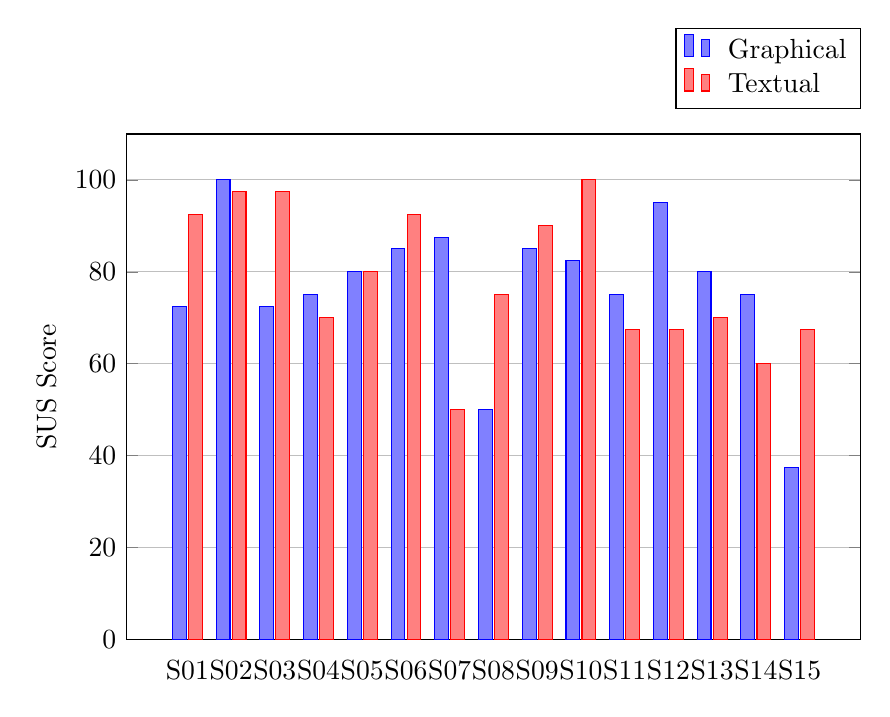
\begin{tikzpicture}
    \begin{axis}[
        width  = 0.90\textwidth,
        height = 8cm,
        major x tick style = transparent,
        ybar=2*\pgflinewidth,
        bar width=5pt,
        ymajorgrids = true,
        ylabel = {SUS Score},
        symbolic x coords={
        S01, S02, S03, S04, S05, S06, S07, S08, S09, S10, S11, S12, S13, S14, S15
        },
        xtick = data,
        scaled y ticks = false,
        % enlarge x limits=0.20,
        ymin=0,
        legend cell align=left,
        legend style={
                at={(1,1.05)},
                anchor=south east,
                column sep=1ex
        }
    ]
        \addplot[style={blue,fill=blue!50}]
            coordinates {
            (S01,72.5) (S02,100) (S03,72.5) (S04,75) (S05,80) (S06,85) (S07,87.5) (S08,50) (S09,85) (S10,82.5) (S11,75) (S12,95) (S13,80) (S14,75) (S15,37.5)
            };

        \addplot[style={red,fill=red!50}]
            coordinates {
            (S01,92.5) (S02,97.5) (S03,97.5) (S04,70) (S05,80) (S06,92.5) (S07,50) (S08,75) (S09,90) (S10,100) (S11,67.5) (S12,67.5) (S13,70) (S14,60) (S15,67.5)
            };
            
        \legend{Graphical,Textual}
    \end{axis}
\end{tikzpicture}
